\texttt{min\_total\_length([1, 2, 3, 7], [0, 4, 5, 9, 10])}

The figure below illustrates this example.

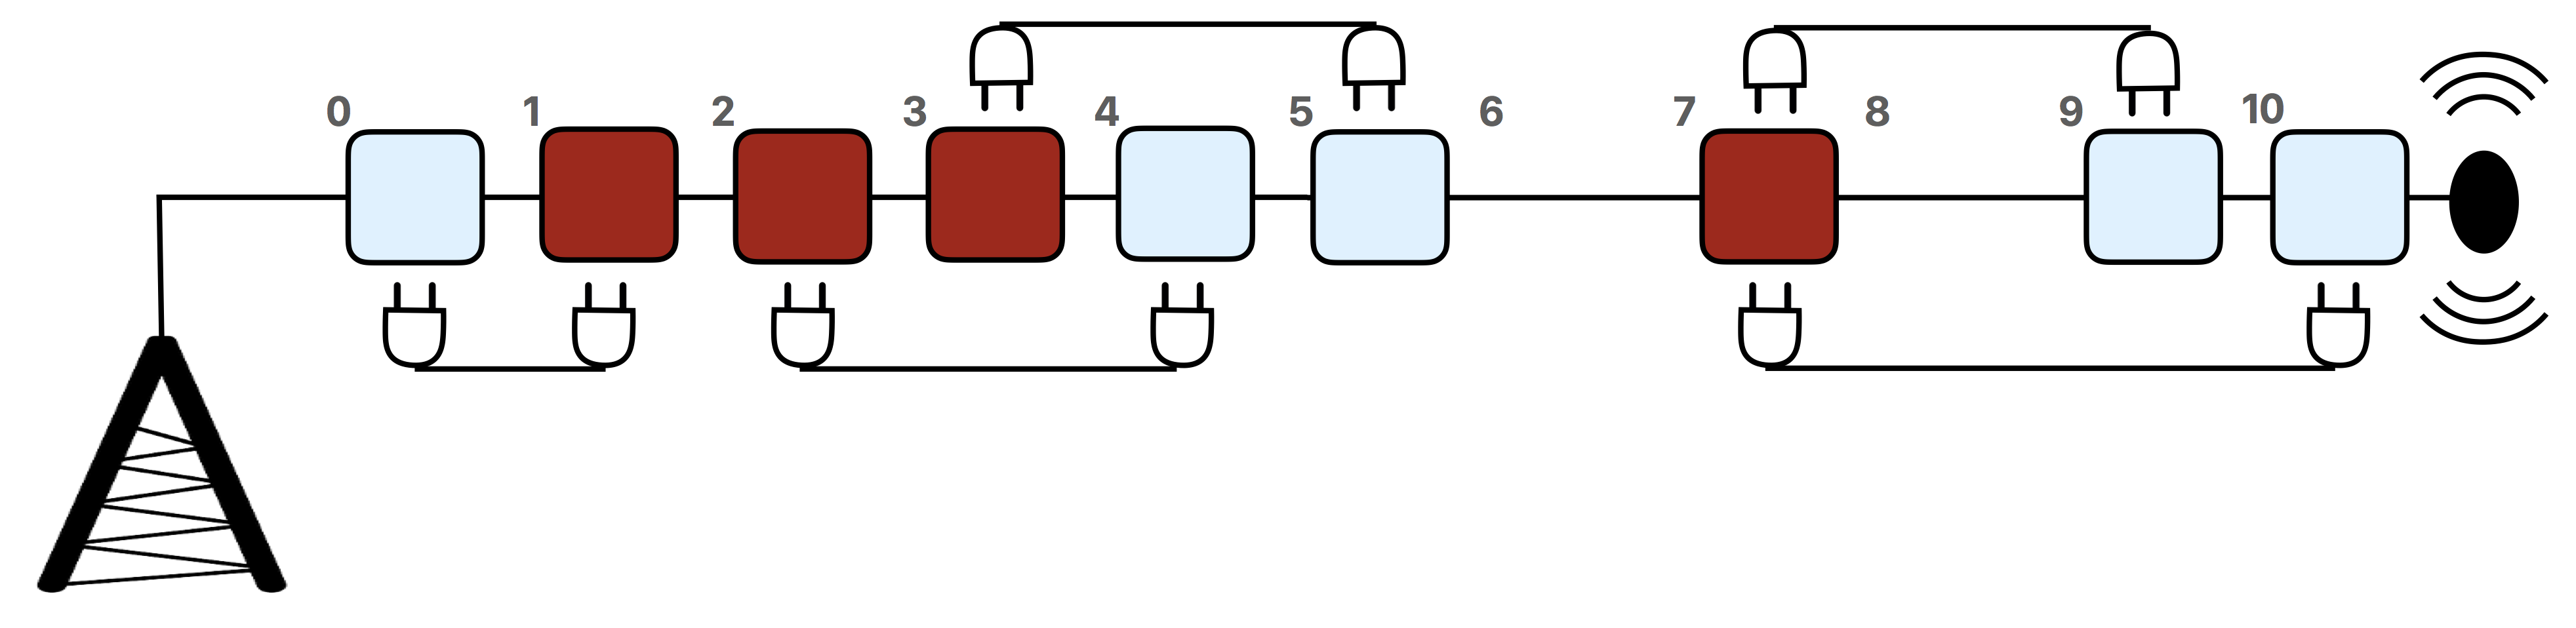
\includegraphics[scale=0.5]{wiring.png}

\begin{itemize}
\item The tower is shown horizontally.
\item In the black-and-white printed version of the problem statement the red connection points are dark and the blue ones are light.
\item There are $4$ red connection points, located at positions $1, 2, 3,$ and $7$.
\item There are $5$ blue connection points, located at positions $0, 4, 5, 9,$ and $10$.
\item One optimal solution is shown in the figure above.
\item In this solution, the total length of the wires is $1 + 2 + 2 + 2 + 3 = 10$, which is optimal. So, the procedure should return $10$.
\item Note that two wires are connected to the connection point at position $7$.
\end{itemize}